\documentclass[a4paper,11pt]{article}
% Various packages
\usepackage{siunitx}
\usepackage[utf8]{inputenc} % æøå
\usepackage[T1]{fontenc} % mere æøå
\usepackage[danish]{babel} % orddeling
\usepackage{verbatim} % så man kan skrive ren tekst
\usepackage{graphicx}
\graphicspath{{assets/}}
\usepackage{a4wide}
\usepackage{url}
\usepackage[left=2cm,top=2cm,bottom=1.5cm,right=2cm]{geometry}
\usepackage{amsmath}
\usepackage{amssymb}
\usepackage{amsthm}
\usepackage{wrapfig}
\usepackage{fixme}
\usepackage{color}
\usepackage{pstricks}
\usepackage{pdfpages} % include pdf
\usepackage{float} % Use [H] in figures
\usepackage{subcaption} % For subfigures
\usepackage{color} % May be necessary if you want to color links
\usepackage{hyperref} % Make references clickable
\usepackage[nameinlink,capitalize]{cleveref} % Make eq:refs be in style (1)
\usepackage[linesnumbered, commentsnumbered, lined, ruled, vlined,
%noend  % Have no ⌊-like symbol to indicate end of scope in pseudocode
]{algorithm2e} % Doc: https://goo.gl/6bC1qZ

% Ændr på navnene der vises når man bruger \autoref{label}
\def\sectionautorefname{Sektion}
\renewcommand{\equationautorefname}{Ligning}
\def\figureautorefname{Figur}
\AtBeginDocument{\renewcommand{\ref}[1]{\autoref{#1}}}

% Sæt \ref{} til at kalde \autoref{}
\AtBeginDocument{\renewcommand{\ref}[1]{\autoref{#1}}}

% Ændr ''*'' i math-felter til \cdot
\DeclareMathSymbol{*}{\mathbin}{symbols}{"01}

% Sæt farver for interne referencer og links
\definecolor{darkblue}{RGB}{25,25,112}
\hypersetup{
	colorlinks=true,    %set true if you want colored links
	linktoc=all,        %set to all if you want both sections and subsections linked
	linkcolor=darkblue, %choose some color if you want links to stand out
	filecolor=blue,     %
	citecolor=black,    %
	urlcolor=cyan,      %
}

% Set indentation to 0:
\setlength\parindent{0pt}

% Keywords relateret til algorithm2e pakken
\newcommand{\True}{\textbf{true}}\newcommand{\False}{\textbf{false}}
\SetStartEndCondition{ }{}{}%
\SetKwProg{Fn}{def}{\string:}{}
\SetKw{KwTo}{to}
\SetKwFor{For}{for}{}{}% 
\SetKwFor{ForEach}{foreach}{}{}% 
\SetKwIF{If}{ElseIf}{Else}{if}{}{elif}{else}{end}% 
\SetKwFor{While}{while}{}{end}\SetKwProg{Fn}{}{}{}
\SetKwInOut{Input}{input}\SetKwInOut{Output}{output}
\setlength{\algomargin}{3em}\DontPrintSemicolon

\newcommand{\longspace}{{\ \ \ \ \ \ \ \ \ \ \ \ \ \ }}
\renewcommand{\P}{{\mathbb P}}
\newcommand{\parfrac}[1]{\frac{\partial}{\partial #1}}
\renewcommand{\num}{{\textrm{num} }}
\newcommand{\size}{{\textrm{size} }}
\newcommand{\ift}{{\textrm{if } }}

% Dynamiske (), <>, ceil, floor
\newcommand{\p}[1]{\left( #1 \right)}
\newcommand{\pbig}[1]{\big( #1 \big)}
\newcommand{\pBig}[1]{\Big( #1 \Big)}
\newcommand{\pbigg}[1]{\bigg( #1 \bigg)}
\newcommand{\larr}[1]{\left< #1 \right>}
\newcommand{\ceil}[1]{\left\lceil #1 \right\rceil}
\newcommand{\floor}[1]{\left\lfloor #1 \right\rfloor}


% Squiggly arrows
\DeclareFontFamily{U} {MnSymbolC}{}

\DeclareFontShape{U}{MnSymbolC}{m}{n}{
	<-6> MnSymbolC5
	<6-7> MnSymbolC6
	<7-8> MnSymbolC7
	<8-9> MnSymbolC8
	<9-10> MnSymbolC9
	<10-12> MnSymbolC10
	<12-> MnSymbolC12}{}
\DeclareFontShape{U}{MnSymbolC}{b}{n}{
	<-6> MnSymbolC-Bold5
	<6-7> MnSymbolC-Bold6
	<7-8> MnSymbolC-Bold7
	<8-9> MnSymbolC-Bold8
	<9-10> MnSymbolC-Bold9
	<10-12> MnSymbolC-Bold10
	<12-> MnSymbolC-Bold12}{}

\DeclareSymbolFont{MnSyC} {U} {MnSymbolC}{m}{n}

\DeclareMathSymbol{\MNrhd}{\mathbin}{MnSyC}{76}
\DeclareMathSymbol{\MNlhd}{\mathbin}{MnSyC}{78}
% =============================================
\DeclareFontFamily{U} {MnSymbolD}{}

\DeclareFontShape{U}{MnSymbolD}{m}{n}{
	<-6> MnSymbolD5
	<6-7> MnSymbolD6
	<7-8> MnSymbolD7
	<8-9> MnSymbolD8
	<9-10> MnSymbolD9
	<10-12> MnSymbolD10
	<12-> MnSymbolD12}{}
\DeclareFontShape{U}{MnSymbolD}{b}{n}{
	<-6> MnSymbolD-Bold5
	<6-7> MnSymbolD-Bold6
	<7-8> MnSymbolD-Bold7
	<8-9> MnSymbolD-Bold8
	<9-10> MnSymbolD-Bold9
	<10-12> MnSymbolD-Bold10
	<12-> MnSymbolD-Bold12}{}

\DeclareSymbolFont{MnSyD} {U} {MnSymbolD}{m}{n}
\DeclareMathSymbol{\MNsim}{\mathbin}{MnSyD}{2}

% =============================================

\usepackage{amssymb,amsmath,stackengine}
\stackMath
\newcommand\rsquigarrow[1]{%
	\mathbin{\stackon[2pt]{\rightsquigarrow}{\scriptscriptstyle #1 }}
}

\author{Søren Mulvad, rbn601}

\title{Eksamensdisposition - Grådige algoritmer}
\begin{document}
\maketitle

% Desuden skal hver studerende i gruppen udarbejde en individuel disposition for emnet "Greedy choice", som er et af emnerne til eksamen. En disposition skal bestå af de vigtigste punkter, du vil komme ind på til eksamen.
% Tænk på dispositionen som noget, du kan have med dig til eksamen, og som kan hjælpe dig med at huske, hvad du overordnet vil gennemgå til emnet "Divide and Conquer".
% Dispositionen skal ikke indeholde detaljerede beviser og lignende, men de mere overordnede delemner. Sørg for at gøre den kortfattet - f.eks. 5-10 punkter med stikord/-sætninger.


\begin{itemize}
	\item \textbf{Paradigmet}
	\item \textbf{Håndkørsel af \texttt{Huffman}}
	\begin{itemize}
		\item Eksempel: \verb|{a:45, d:16, b:13, c:12, e:9, f:5}|
	\end{itemize}
	\item \textbf{Bevis af korrekthed af \texttt{Huffman}}
	\begin{itemize}
		\item Redegørelse for Lemma omkring summen af frekvenser
		\item Greedy choice property
		\item Optimal delstruktur
	\end{itemize}
\end{itemize}




%%%%%%%%%%%%%%%%%%%%%%%%%%%%%%%%%%%%%%%%%%%%%%%%%%%%%%%%%%%
%%%%%%%%%%%%%%%%%%%%%%%%%%%%%%%%%%%%%%%%%%%%%%%%%%%%%%%%%%%
%%%%%%%%%%%%%%%%%%%%%%%%%%%%%%%%%%%%%%%%%%%%%%%%%%%%%%%%%%%
\newpage
%%%%%%%%%%%%%%%%%%%%%%%%%%%%%%%%%%%%%%%%%%%%%%%%%%%%%%%%%%%
%%%%%%%%%%%%%%%%%%%%%%%%%%%%%%%%%%%%%%%%%%%%%%%%%%%%%%%%%%%
%%%%%%%%%%%%%%%%%%%%%%%%%%%%%%%%%%%%%%%%%%%%%%%%%%%%%%%%%%%
\section{Grådige algoritmer}





\textbf{Paradigmet}

\begin{itemize}
	\item Grådige algoritmer minder en smule om dynamisk programmering, i og med vi har en række delproblemer der afhænger af løsningen på andre delproblemer.
	\item Forskellen er, at med en grådig algoritme laver vi altid den løsning som på nuværende tidspunkt ser bedst ud, uden at kigge på fremtidige delproblemer.
	\item Hermed laver vi en lokal optimal løsning, som vi håber vil lede til en global optimal løsning. 

\item \textbf{Egenskaber for problemerne:}\\
\textit{Greedy choice property:}\\
Vil sige at vi kan samle en global optimal løsning ved at lave lokale optimale (grådige) valg. Altså, når vi beregner hvilket valg vi skal tage, kan vi tage det valg som er bedst for det nuværende problem uden at tage højde for løsningerne til delproblemerne. Hermed får vi hele tiden et lignende, men mindre, delproblem.\\



\textit{Optimal delstruktur:}\\
Vise sige, at hvis der fandtes en optimal løsning der indeholder det grådige valg, så består den optimale løsning af det grådige valg + en løsning til det delproblem vi har tilbage når vi har lavet det grådige valg.\\


%\item \textbf{Design af grådig algoritme:}
%\begin{enumerate}
%	\item Lav problemet om til et problem hvor vi tager et valg og har et delproblem tilbage at løse.
%	\item Bevis at der altid er en optimal løsning til det originale problem som laver det grådige valg, så det grådige valg er altid sikkert.
%	\item Demonstrer optimal substruktur ved at vise, at ved at have lavet det grådige valg er det vi er efterladt med et delproblem der har den egenskab, at hvis vi kombinerer den optimale løsning til delproblemet med det grådige valg, så får vi en optimal løsning til det originale problem.
%\end{enumerate}

\item Eksempler på grådige algoritmer er activity-selection, Dijkstras algoritme og Huffman-koder. Jeg vil her gå mere i dybden med Huffman-koder.
\end{itemize}


\textbf{Håndkørsel af \texttt{Huffman}}
\begin{itemize}
	\item Løser problemet med at vi gerne vil sende noget information, men ønsker at gøre brug af, at der er en hvis redundans i informationen. Ved at kode de karakterer der optræder flest gange med den laveste kode får vi den mindst mulige filstørrelse. Men hvordan finder vi ud af, hvordan vi skal kode dem, så vi overholder dette samtidig med at slutkodningen ikke kan tolkes på flere måder?
	\item Vi indfører følgende notation:
	\begin{itemize}
		\item $T$ er et parse-træ for en præfikskode.
		\item $C$ er sættet af karakterer, f.eks. $C = \{a, b, c, d, e, f\}$. For hver karakter $c \in C$ har vi:
		\item $f_c$ for frekvensen af denne karakter.
		\item $d_T(c)$ for dybden af bladet i $T$.
		\item $B(T) = \displaystyle\sum_{c \in C} f_c * d_T(c)$ er omkostningen af træet. Vi ønsker naturligvis at minimere $B(T)$.
	\end{itemize}
	\item Algoritmen virker ved at tage de to elementer med lavest frekvens og sætte dem sammen så de bliver søskende i et deltræ med en forælder der har en frekvens som er summen af dens børn. Dette gør algoritmen $n-1$ gange, så alle knuder til sidst er sat sammen til et og samme deltræ.
	\begin{figure}[H]
		\begin{center}
			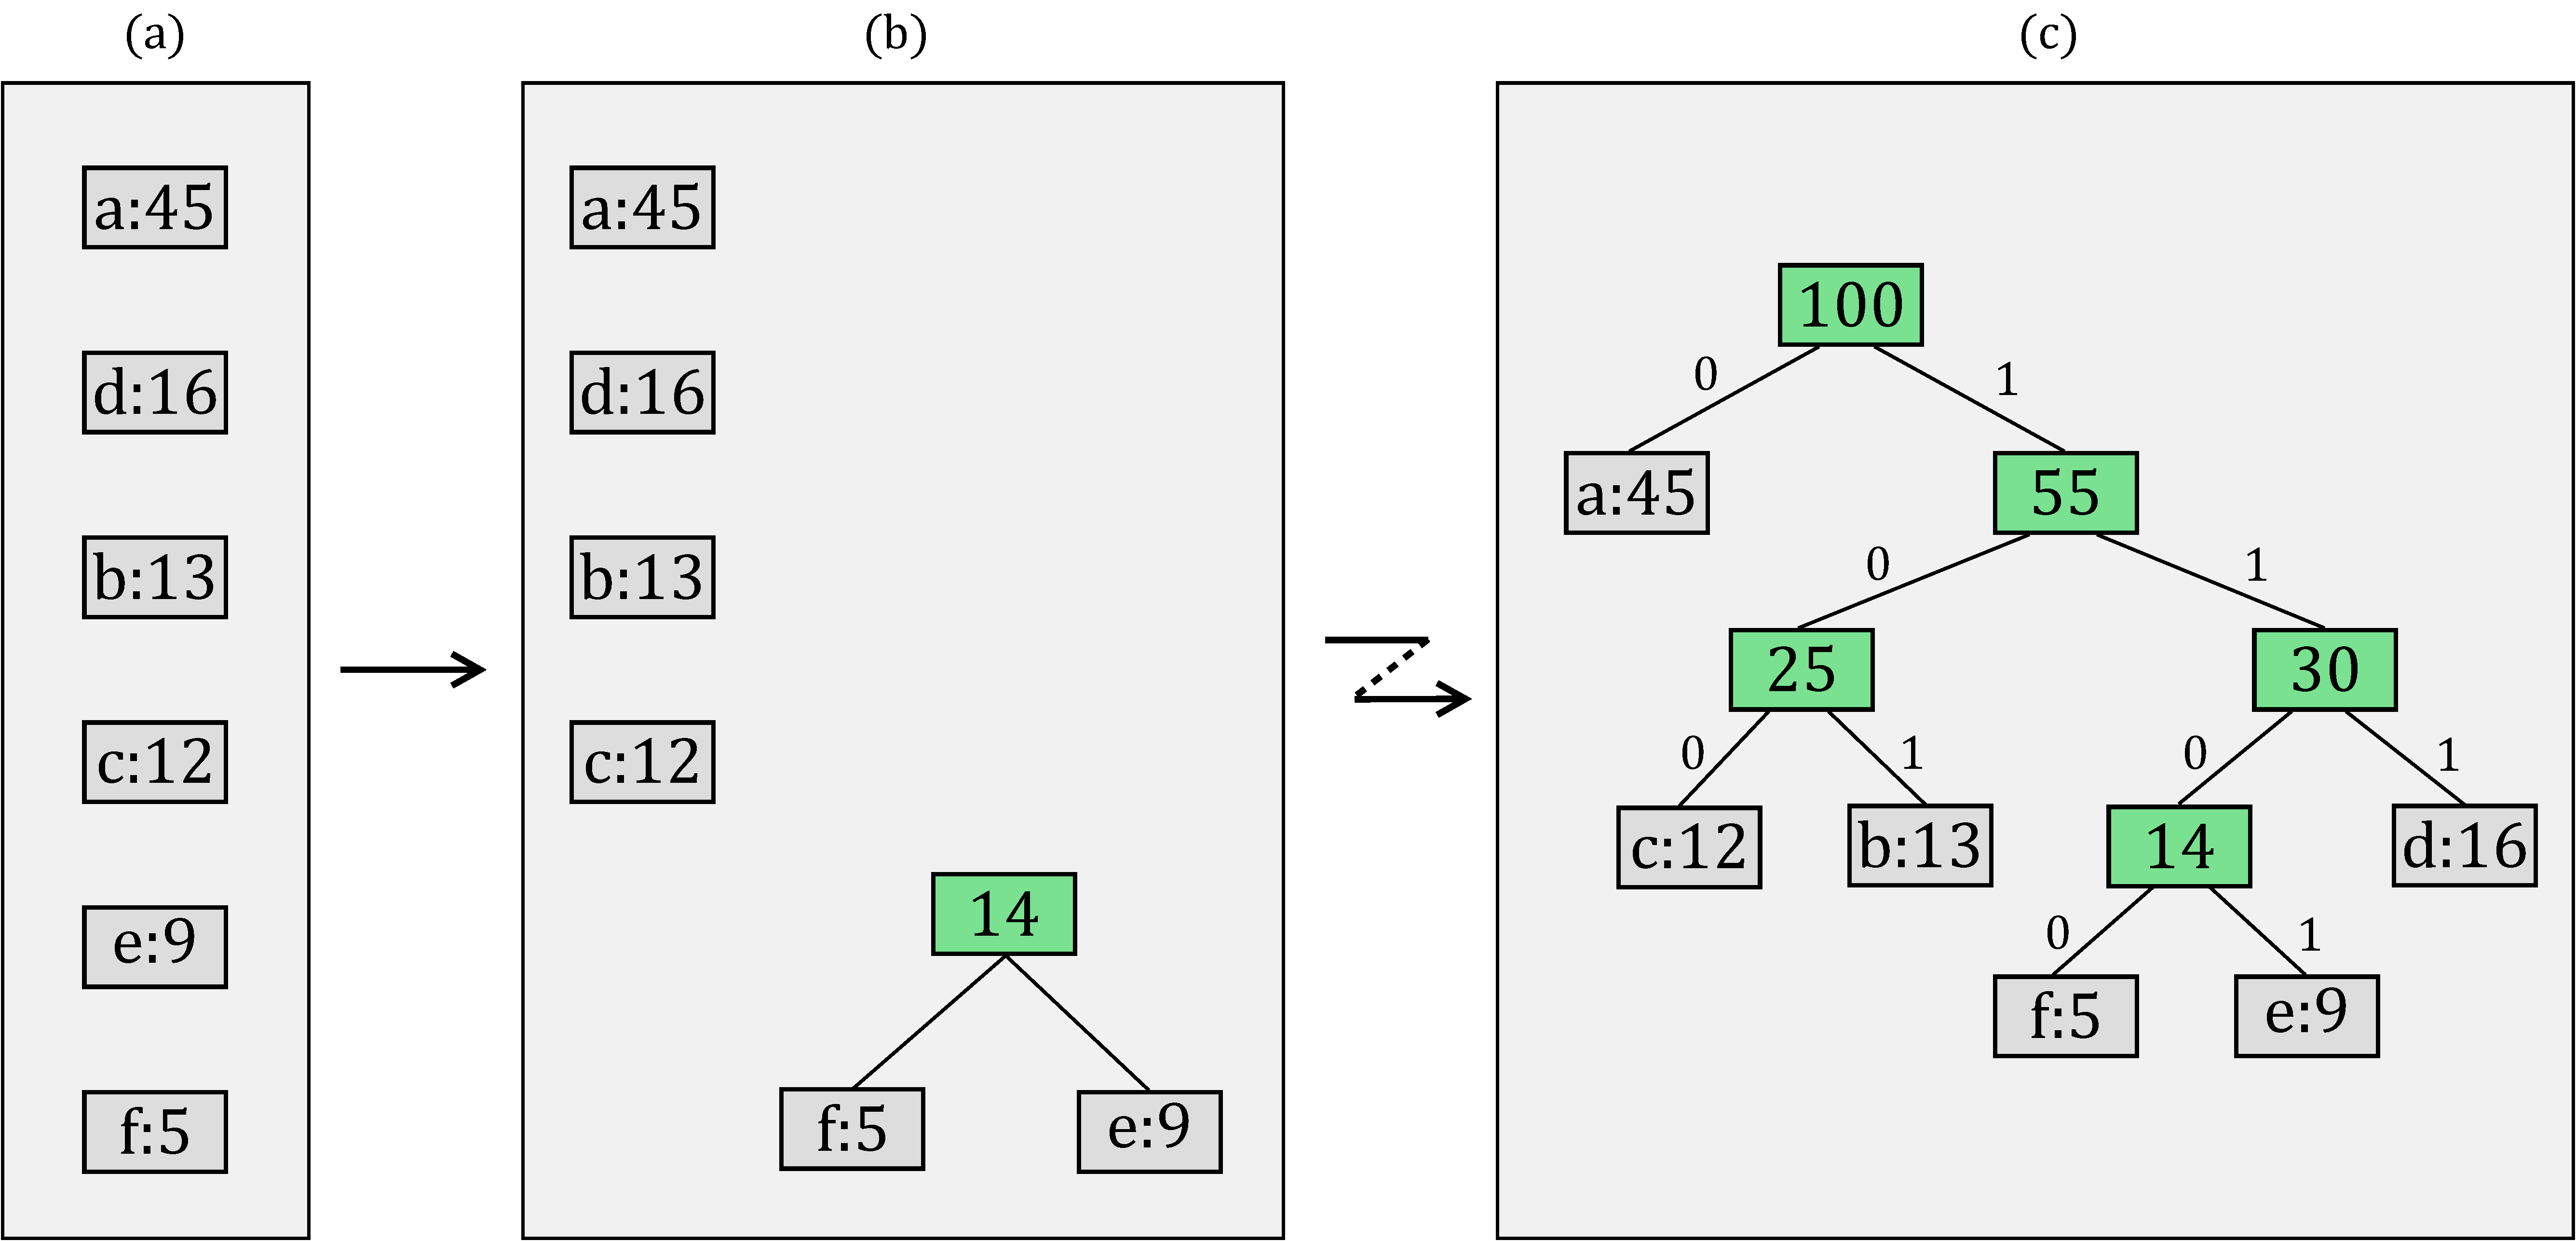
\includegraphics[width=\textwidth]{haandkoersel.pdf}
		\end{center}
		\caption{
		\textbf{(a)} Algoritmen idet alle karakterer $c \in C$ er sat ind i vores datastruktur, men inden vi har kørt nogle iterationer.\\
		\textbf{(b)} Algoritmen efter første iteration, hvor vi vælger $f$ og $e$ fordi de har lavest frekvens. De sættes sammen og der laves en forældreknude med frekvensen $f_f + f_e = 5+9=14$.\\
		\textbf{(c)} Algoritmen efter alle $n-1$ iterationer af for-loopet er kørt og vi har vores færdige parse-træ $T$. Nu ville bitrepræsentationen for f.eks. $a=0$ og $f = 1100$.}
		\label{fig:haandkoersel}
	\end{figure}
	\item Køretiden afhænger af hvor hurtigt vi kan finde elementet med lavest frekvens og tage det ud, samt hvor hurtigt vi kan indsætte nye elementer. Hvis vi f.eks. bruger Fibonacci Heaps kan vi både køre \texttt{Extract-Min} og \texttt{Insert} i $O(\lg n)$ tid.\\
	Vi ser derudover, at for hver iteration fjerner vi to elementer og tilføjer et, altså er der netto ét element mindre at håndtere hver gang, hvorved vi får $\Theta(n)$ iterationer. Således bliver den totale køretid:
	$$
	O(n \lg n)
	$$
\end{itemize}





\textbf{Bevis af korrekthed af \texttt{Huffman}}\\
Vi har lige bestemt et parse-træ $T$ ved at bruge Huffmans algoritme. Nu vil jeg gerne bevise, at $B(T)$ er minimal. Vi skal bruge et Lemma jeg ikke decideret vil bevise, men som giver god mening ud fra \ref{fig:haandkoersel}.\\

\textit{Lemma:} Hvis vi lader $W$ være alle knuder pånær roden, så har vi for ethvert parse-træ $T$ at:
$$
B(T) = \sum_{c \in C} f_c * d_T(c) = \sum_{v \in W} f_v
$$
Dvs. vores frekvens-dybde sum er lig summen af alle frekvenserne af knuder der ligger i $W$. Se f.ek.s på (c) i \ref{fig:haandkoersel}.\\


For nu at bevise, at \texttt{Huffman} giver en optimal præfikskode skal vi vise greedy choice property og optimal delstruktur.\\







\textbf{Greedy choice property:}\\
Vi skal altså vise, at det grådige valg er med i mindst en af de optimale løsninger. Dvs. når vi finder de to symboler med lavest frekvens, sætter dem sammen, og giver dem en fælles forælder, så findes der en optimal løsning som har de her to knuder med mindst frekvens som søskendeblade i den optimale løsning.

Lad os kalde de to karakterer med lavest frekvens for $x$ og $y$.\\

Vi har greedy choice property fra det faktum, at et optimalt træ $OPT$ kan blive transformeret om til et andet træ $OPT'$ som har det grådige valg (at $x$ og $y$ er søskendeblade):

\begin{figure}[H]
	\begin{center}
		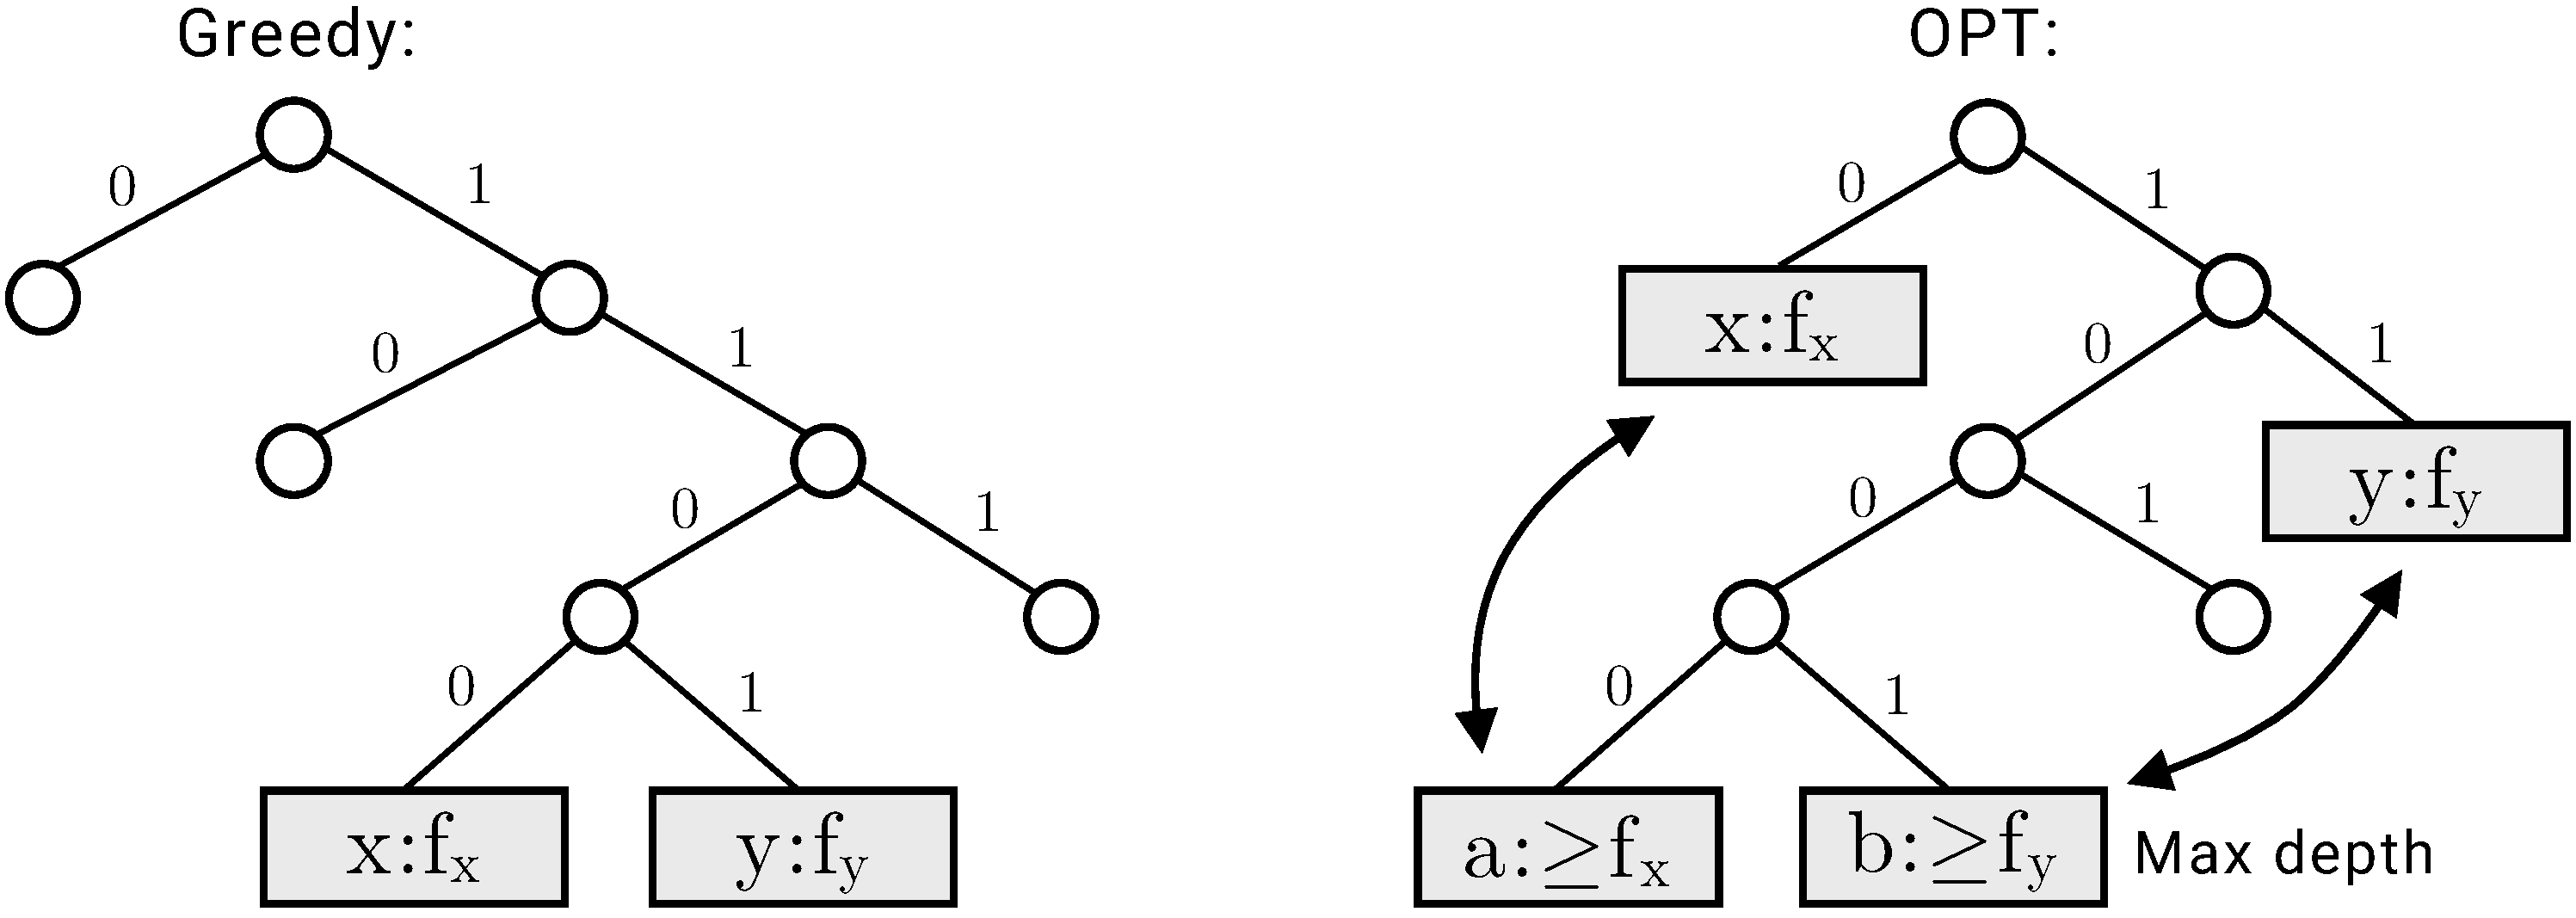
\includegraphics[width=\textwidth]{greedy-choice.pdf}
	\end{center}
	\caption{Bemærk der med $a$ og $b$ i ulighederne i figuren menes frekvensen af de to, altså $f_a$ og $f_b$}
	\label{fig:greedy-choice}
\end{figure}

På \ref{fig:greedy-choice} har vi først outputtet fra \texttt{Huffman} (dvs. $x$ og $y$ er søskendeblade) og derefter et arbitrært optimalt træ $OPT$. Men $OPT$ kan vi nu lave om til et nyt træ $OPT'$ der også har det grådige valg. Det kan vi, fordi ulighederne på figuren gælder da vi netop har defineret $x$ og $y$ til at være de elementer med henholdsvis lavest og næstlavest frekvens.\\

Frekvensen af $a$ er mindst lige så stor som frekvensen af $x$. Så ved at flytte $a$ op kan vi få en kortere bitrepræsentation til noget der optræder lige så mange gange eller hyppigere end $x$. Her ses et formelt bevis, hvor $OPT = T$ er træet før ombytningen og $OPT' = T'$ er træet efter ombytningen af $x$ og $y$:

\begin{alignat}{2}
B(T') &= B(T) &&- f_a * d_{T}(a) - f_x * d_{T}(x) \nonumber \\
      &       &&+ f_a * d_{T}(x) + f_x * d_{T}(a) \label{eq:start} \\
      &= B(T) &&+ \underbrace{(f_a - f_x)}_{\geq 0} \underbrace{(d_T(x) - d_T(a))}_{\leq 0} \label{eq:parenteser} \\
      &\leq B(T) && \Longrightarrow \text{$T'$ er optimal}  \label{eq:res}
\end{alignat}

\begin{enumerate}
	\item[Eq. \cref{eq:start}] Vi ved, at omkostningen af træet $T'$ hvor $x$ byttes med $a$ svarer det til det gamle træ, og hvor vi så tager højde for de ændringer vi laver. Vi tager udgangspunkt i det optimale træ $T$ i alle led.
	\item[Eq. \cref{eq:parenteser}] Vi sætter de to frekvenser sammen til et led samt de to dybder til et led. Det første led er $\geq 0$ da det er vores antagelse jf. vores greedy choice property. Det andet led er $\leq 0$, da vi valgte $a$ til at have maksimal dybde.
	\item[Eq. \cref{eq:res}] Vi ser, at vi muligvis ganger et positivt med et negativt tal, og derfor må det led totalt blive $\leq 0$. Således får vi $B(T') \leq B(T)$, som medfører at $T'$ er optimal.
\end{enumerate}

Altså har vi nu vist, at det grådige valg hvor $x$ og $y$ er søskendeblade er med i mindst en af de optimale løsninger.






\newpage
\textbf{Optimal delstruktur:}\\
Det vi nu vil vise er, at hvis der fandtes en optimal løsning der indeholder det grådige valg, så består den optimale løsning af det grådige valg + en løsning til det delproblem vi har tilbage når vi har lavet det grådige valg.\\

Det delproblem vi har tilbage er et nyt alfabet $C' = (C \ \backslash \ \{x, y\}) \cup \{z\}$, altså hvor vi har fjernet $x$ og $y$ fra det oprindelige problem og indsat en ny ''karakter'' $z$ med $f_z = f_x + f_y$.\\

Nu skal vi vise, at hvis det grådige valg er i et optimalt træ $T_1$ for $C$, så er $T_1' = T_1 \ \backslash \ \{x, y\}$ et optimalt træ for $C'$.

Derudover indfører vi $T_2'$, som er en optimal løsning til vores problem med det reducerede alfabet $C'$, og $T_2 = T_2' \cup \{x, y\}$ som er den optimale løsning med søskendebladene. 
\begin{figure}[H]
	\begin{center}
		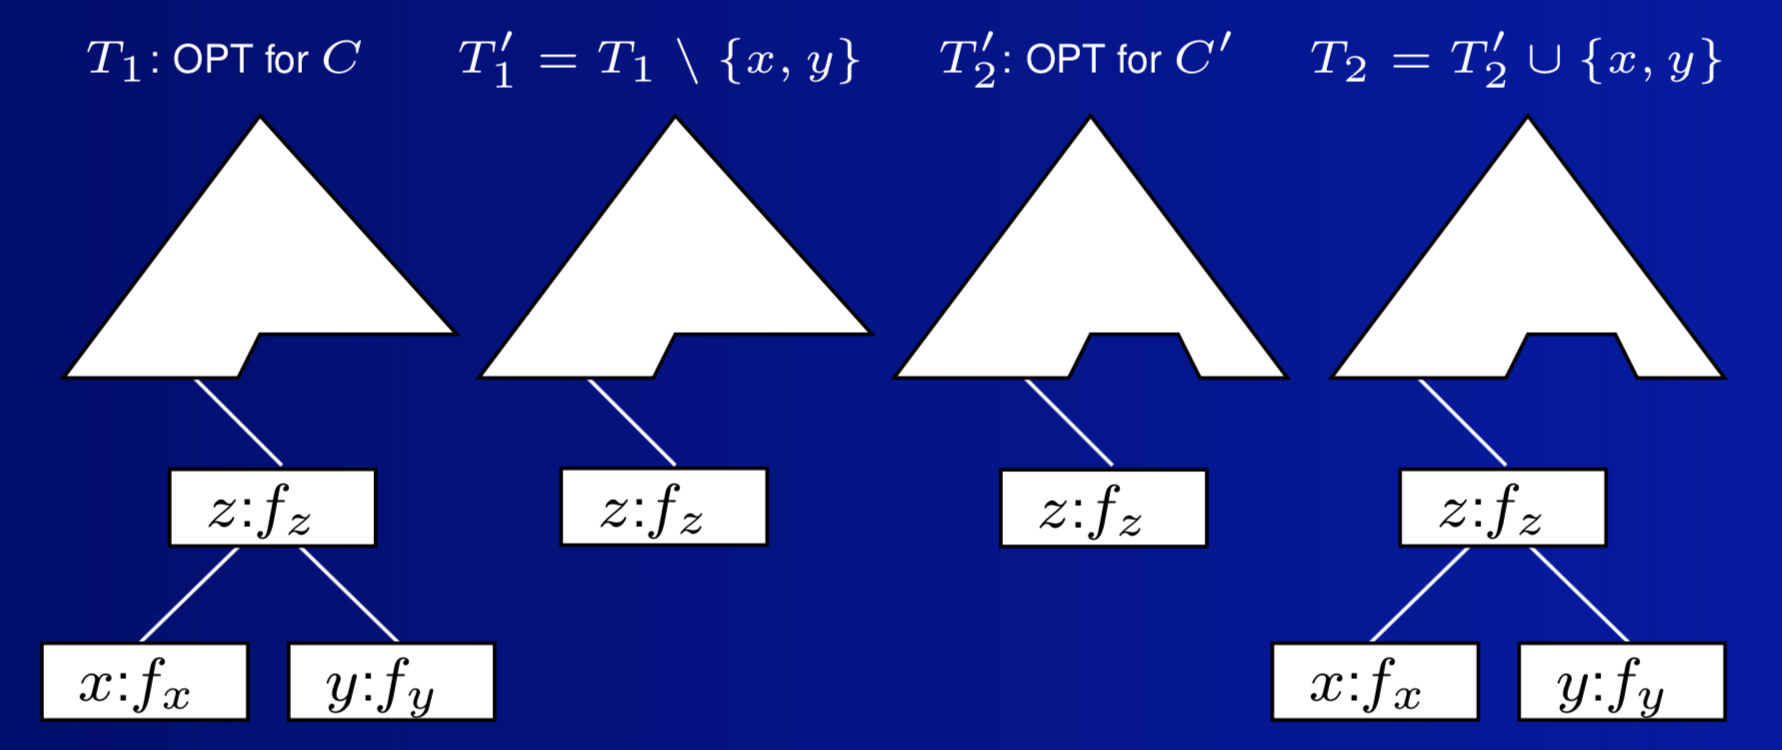
\includegraphics[width=\textwidth]{opt-sub.png}
	\end{center}
	%\caption{caption}
	\label{fig:opt-sub}
\end{figure}

Vi ønsker at vise, at $B(T_1') \leq B(T_2')$, da $T_2'$ netop er defineret til at være en optimal løsning for delproblem $C'$. Ved at vise dette viser vi nemlig, at delløsningen $T_1'$ faktisk er en optimal løsning for $C'$.\\

Fra figuren ser vi:
$$
B(T_1') = B(T_1) - f_x - f_y \leq B(T_2) - f_x - f_y = B(T_2')
$$
Lighederne gælder, da vi jf. vores Lemma ved at $B(T)$ er lig summen af frekvenserne af alle knuder pånær roden.\\

Uligheden gælder, da vi definerede at $T_1$ er en optimal løsning til $C$.\\


\end{document}